\documentclass{article}
\usepackage{listings}
\usepackage{color}
\usepackage{float}
\usepackage{graphicx}

\definecolor{dkgreen}{rgb}{0,0.6,0}
\definecolor{gray}{rgb}{0.5,0.5,0.5}
\definecolor{mauve}{rgb}{0.58,0,0.82}

\lstset{
	frame=single,
	language=C,
	belowskip=3mm,
	showstringspaces=false,
	columns=flexible,
	captionpos=b,
	basicstyle={\small\ttfamily},
	numbers=left,
	numbersep=5pt,
	%numbers=none,
	numberstyle=\tiny\color{gray},
	keywordstyle=\color{blue},
	commentstyle=\color{dkgreen},
	stringstyle=\color{mauve},
	breaklines=true,
	breakatwhitespace=true,
	tabsize=4
}

\input kvmacros
\sloppy
\begin{document}

\title{Project 1: Compile Linux Kernel}
\author{\textit{Yesheng Ma}}
\date{\today}
{\bf\small CS353: Linux Kernel}\hfill{\bf\small 2017 Spring}
{\let\newpage\relax\maketitle}
\maketitle


\begin{abstract} 
The configuration, compilation, and installation of the Linux kernel is the first step to learn Linux kernel. In this report, I will discuss how to get Linux source code and get the latest kernel installed on your PC.
\end{abstract}


\section{Introduction}
Linux kernel is an operating system kernel, which is written in C and assembly language originally by Linus Torvalds. The latest stable version of Linux is 4.10 and is licensed under GPLv2. In this project, we will begin our tour in Linux kernel, where we will build and install the latest kernel in a PC or virtual machine.

\section{Obtain Linux Kernel Source}
We can obtain Linux source code both in the form of git repository or through HTTP. The official site of the Linux kernel is \texttt{https://www.kernel.org}. For example, you can download the latest kernel source code in the \texttt{.tar.xz} form using \texttt{wget} or using \texttt{git clone} to copy the whole repository.

\begin{figure}[H]
\centering
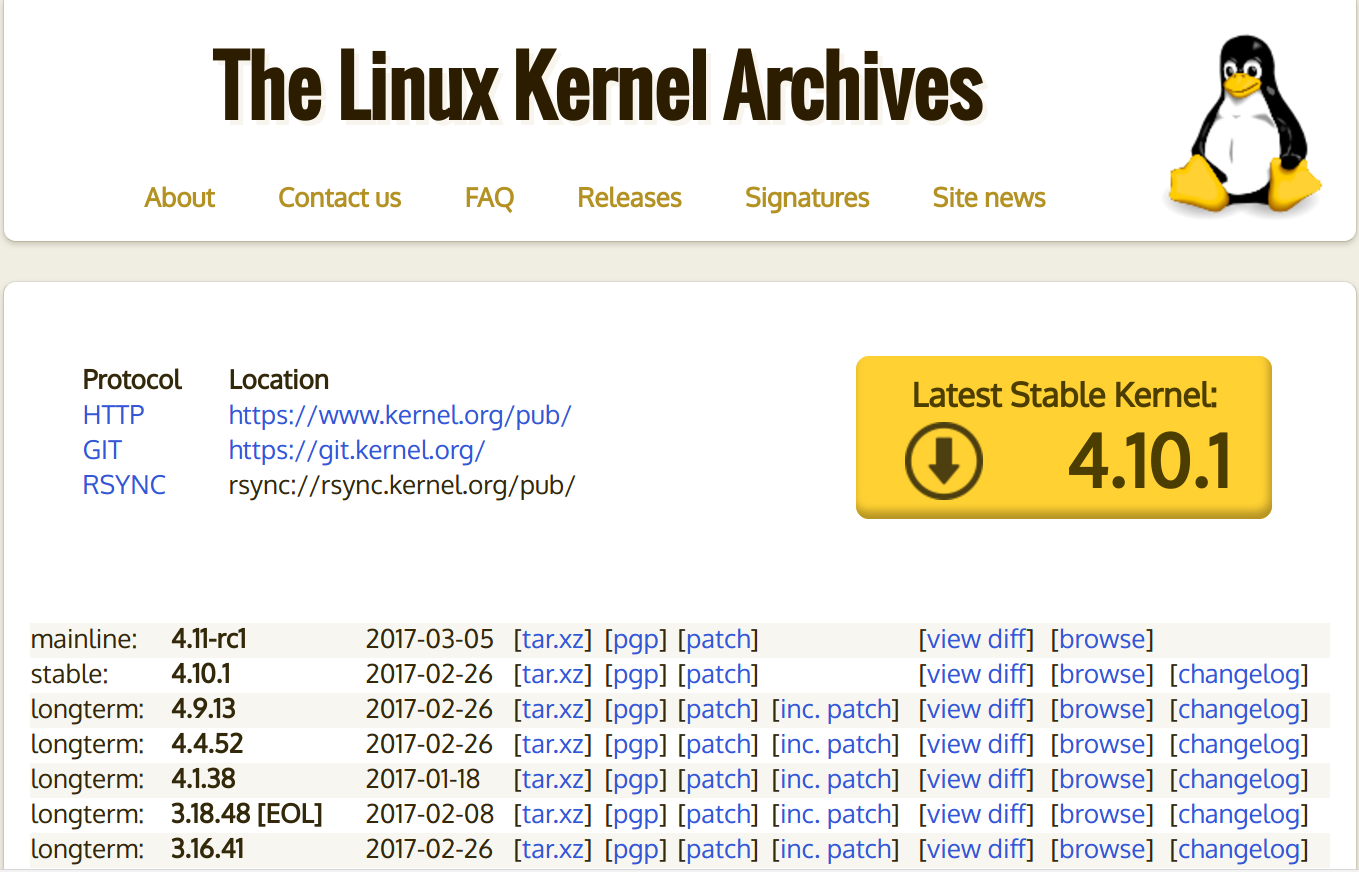
\includegraphics[width=7cm]{website.png}
\caption{Linux Kernel Official Site}
\end{figure}
  
After you have downloaded the \texttt{tar.xz} file, you can extract the file using the command \texttt{tar --xz -xvf}.
\begin{figure}
\centering
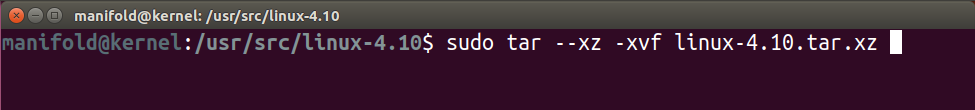
\includegraphics[width=8cm]{tar.png}
\caption{Extract the tar file}
\end{figure}
Then we can check out the files extracted in the source directory.
\begin{figure}[H]
\centering
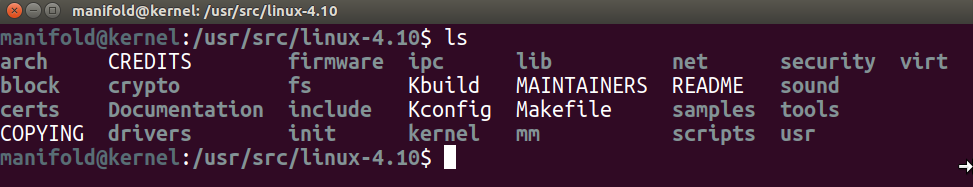
\includegraphics[width=8cm]{dirs.png}
\caption{Linux Source File Directory}
\end{figure}

\section{Build the Kernel}
\subsection{Configure the Kernel}
To compile the kernel, you need to first do some configurations to it. The most often used configuration tool is called \texttt{menuconfig}. Type \texttt{make menuconfig} in the source directory and the default setting should be fine for us.
\subsection{Compile the Kernel}
First we should compile the C and assembly source code to binary form. To do this, simply execute \texttt{make} in the source directory.
\begin{figure}[H]
\centering
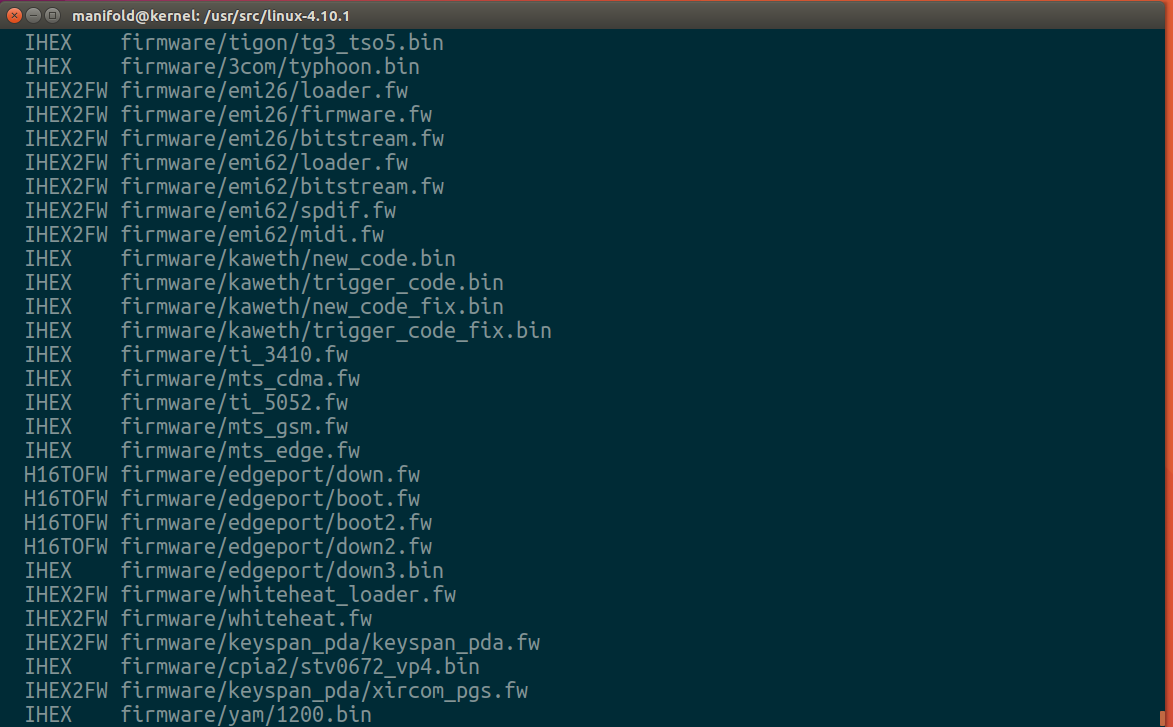
\includegraphics[width=8cm]{make.png}
\caption{Making the Kernel}
\end{figure}
Then we should install the modules using \texttt{make modules\_install}.
\begin{figure}[H]
\centering
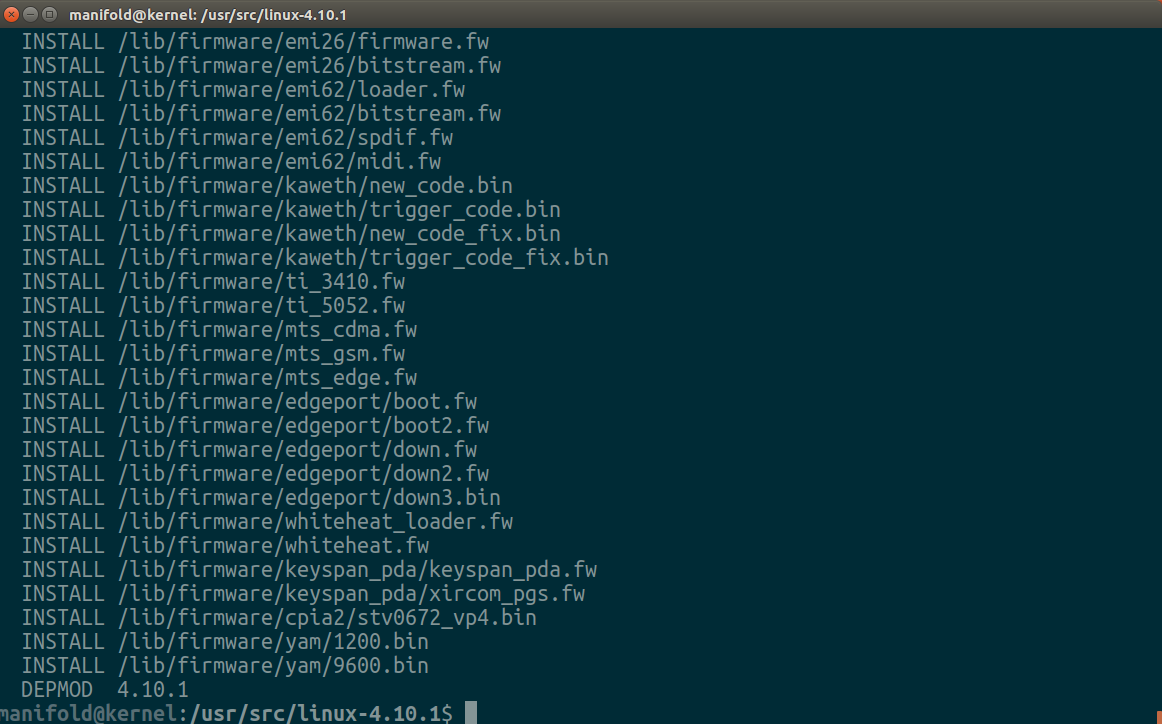
\includegraphics[width=8cm]{makemod.png}
\caption{Make Kernel Model}
\end{figure}
Last, we need to install the kernel image to desired location. To do this, simply execute \texttt{make install} (may need sudo permission).
\begin{figure}[H]
\centering
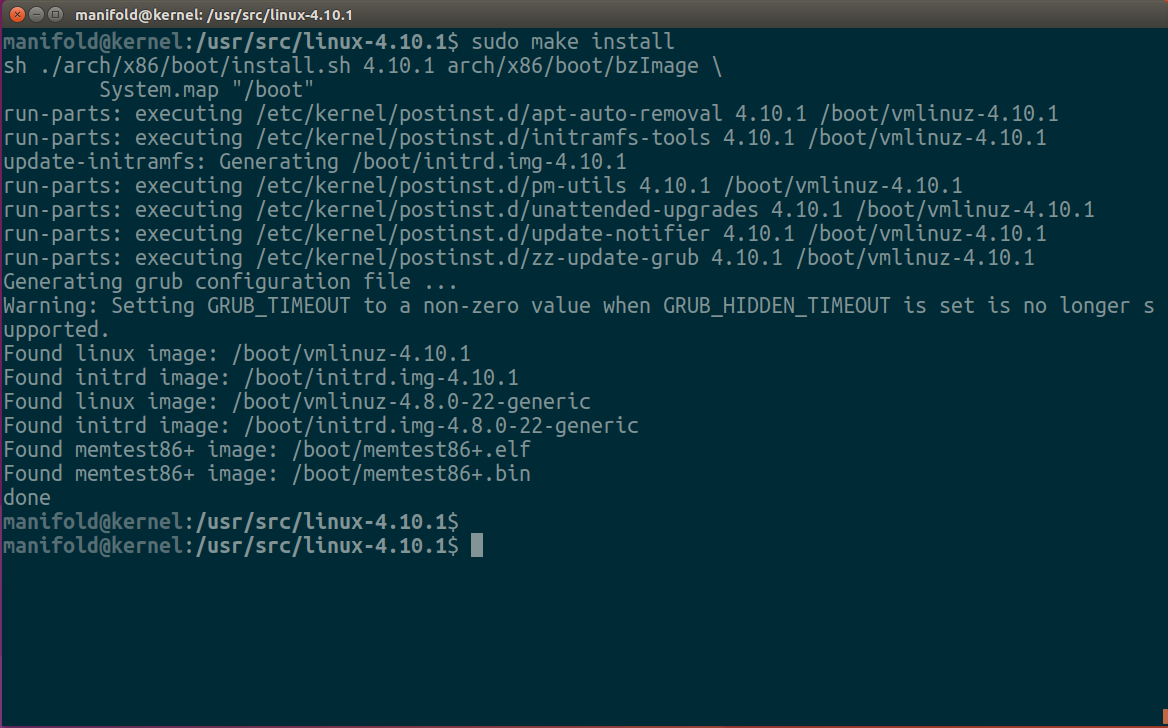
\includegraphics[width=8cm]{makeinstall.png}
\caption{Install the Kernel}
\end{figure}

\section{Change Boot Configuration}
Since we are using Ubuntu 16.10 Linux distribution, we need to configure the Grub boot manager in order to boot from the new kernel. To do this, execute the command \texttt{sudo update-grub2}.
\begin{figure}[H]
\centering
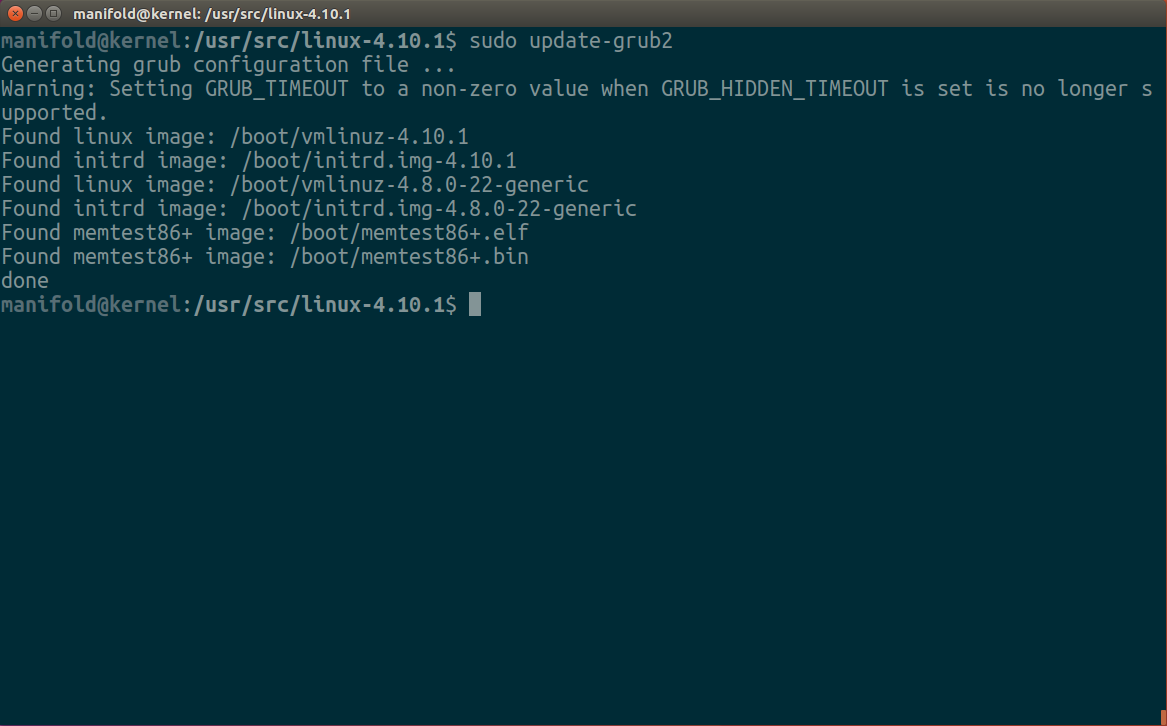
\includegraphics[width=8cm]{grub.png}
\caption{Update Grub Boot Info}
\end{figure}

\section{Checkout New Kernel}
After we reboot the computer, we can checkout the kernel version of the system using \texttt{uname -a}.
\begin{figure}[H]
\centering
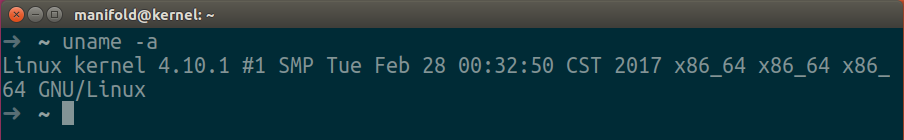
\includegraphics[width=8cm]{uname.png}
\caption{New Kernel Info}
\end{figure}
As we can see in this figure, we can see that we have successfully transferred to Linux 4.10.

\section{Conclusion}
This is the first project on Linux kernel. Although this is a quite simple project: only compile the kernel, I hope it will be a good start for my hacking in Linux kernel.


\section*{Acknowledgement}
Thanks Prof. Chen for guidance on Linux kernel and TAs for their hard work.
\end{document}
